%************************************************
\chapter{Array Heap Allocation}\label{ch:HeapAlloc}
%************************************************

When doing the expansion, we need to create and allocate new arrays. Polly was already able to generate necessary array creation code, if that array has to be located on the stack as part of the pattern-based optimization of matrix multiplication. However, array allocation on the heap, which provides the amount of memory needed for full static array expansion was not possible before.

Consider the following code as an example:
\begin{lstlisting}[frame=single]
for (int i = 0; i < N; i++)
  for (int j = 0; j < N; j++)
    for (int k = 0; k < N; k++)
      for (int l = 0; l < N; l++)
        A[l] = 3;
\end{lstlisting}

The expansion would lead to the following code :
\begin{lstlisting}[frame=single]
for (int i = 0; i < N; i++)
  for (int j = 0; j < N; j++)
    for (int k = 0; k < N; k++)
      for (int l = 0; l < N; l++)
        A_exp[i][j][k][l] = 3;
\end{lstlisting}

Depending on the value of N, $A_{exp}$ can have a huge number of elements. If N = 100, we have $100*100*100*100 = 100000000 = 10^8$ elements ! Thus, the possibility to allocate array on heap was needed.

On the implementation side, special care had to be taken to get the memory allocation/deallocation correct. As opposed to stack-arrays which get freed automatically, heap allocated arrays require explicit calls to malloc and free. As Polly already guards the code that is generated during the execution of its’ optimization pipeline behind a branch, we have chosen to specifically create BasicBlocks right after the branch and right before the join to place our calls to malloc and free for any array that needed to be created on the heap. These two blocks can be seen on Figure~\ref{fig:HeapAllocPlace}.

\begin{figure}
\centering
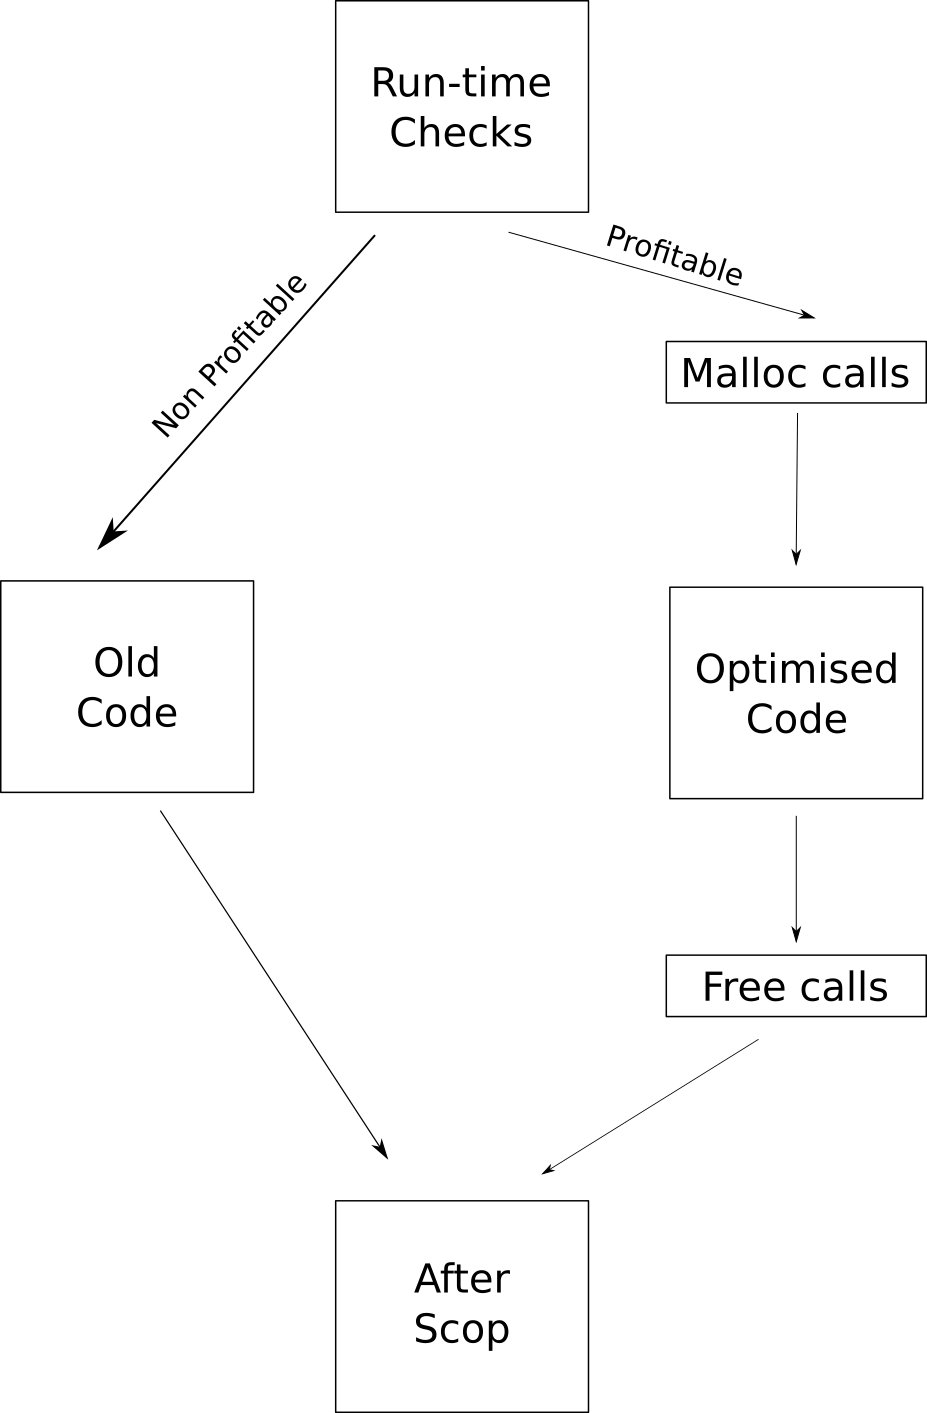
\includegraphics[scale=0.3]{gfx/HeapAlloc/ScopSplit.png}
\caption{Malloc/Free block positions}
\label{fig:HeapAllocPlace}
\end{figure}

As an incremental step, this could be tested via the JSON Importer. We concluded to this solution after long discussion with the Polly community to ensure that we do not risk a use after free error with the newly added arrays. Even if the SCoP is inside a loop, every allocated arrays we'll be freed. This solution is simple to implement but need a mechanism of copy-in/out. This problem will be discussed in Section~\ref{ch:CopyInOut}}.

Technically speaking, to insert malloc and free calls, we used the method described in Section~\ref{ch:LLVM}. Here is a simplified version of the code actually in place :
\begin{lstlisting}[frame=single]
// Get the IntPtrTy from the Datalayout
auto IntPtrTy = DL.getIntPtrType(Ctx);

// Get the size of the element type in bits
unsigned Size = SAI->getElemSizeInBytes();

// Insert the malloc call at polly.start
auto InstIt = std::get<0>(StartExitBlocks)->getTerminator();
auto *CreatedArray = CallInst::CreateMalloc(
          &*InstIt, IntPtrTy, SAI->getElementType(),
          ConstantInt::get(Type::getInt64Ty(Ctx), Size),
          ConstantInt::get(Type::getInt64Ty(Ctx), ArraySizeInt), nullptr,
          SAI->getName());

SAI->setBasePtr(CreatedArray);

// Insert the free call at polly.exiting
CallInst::CreateFree(CreatedArray,
          std::get<1>(StartExitBlocks)->getTerminator());
\end{lstlisting}
Polly.start and Polly.exiting are respectively the first and the last BasicBlock of the Polly branch. These two BasicBlock are passed to this section of code via the pair \emph{StartExitBlocks}.
First, we create the malloc call :
\begin{lstlisting}[frame=single]
// Get the IntPtrTy from the Datalayout
auto IntPtrTy = DL.getIntPtrType(Ctx);

// Get the size of the element type in bits
unsigned Size = SAI->getElemSizeInBytes();

// Insert the malloc call at polly.start
auto InstIt = std::get<0>(StartExitBlocks)->getTerminator();
auto *CreatedArray = CallInst::CreateMalloc(
          &*InstIt, IntPtrTy, SAI->getElementType(),
          ConstantInt::get(Type::getInt64Ty(Ctx), Size),
          ConstantInt::get(Type::getInt64Ty(Ctx), ArraySizeInt), nullptr,
          SAI->getName());
\end{lstlisting}
There are multiple parameters but this call is pretty easy. The first parameter is the instruction before which to insert the call. The second is the type of a int pointer on the machine, we take the one from the DataLayout, a structure containing information about target. The next one is the type of element in the array. The 4th and 5th parameters are the size of one element and the total size of the array (product of all dimensions).

The free call is even more simple :
\begin{lstlisting}[frame=single]
// Insert the free call at polly.exiting
CallInst::CreateFree(CreatedArray,
          std::get<1>(StartExitBlocks)->getTerminator());
\end{lstlisting}
We get from CreateMalloc a pointer to the allocated memory. The CreateFree method take this pointer and the location where to insert the free. And that's all !

The finished support for heap allocation was committed into Polly and all discussion about it can be found \footurl{https://reviews.llvm.org/D33688}{here}.